\chapter{DATA AND MODEL}
\label{ch:data}

\section{Data}

This section presents the observational datasets used as a reference for evaluating the model forecasts. The selected datasets, described in detail in Sections \ref{section311} to \ref{section315}, are commonly employed in tropical cyclone studies and provide reliable information on storm trajectory, intensity, and precipitation. They have been used in several studies \cite{zhou2021regionalization, bopape2021sensitivity, dulac2024assessing, yang2024evaluation, may2024cnn} and support a robust assessment of the model's performance

\subsection{IBTrACS}
\label{section311}

The International Best Track Archive for Climate Stewardship (IBTrACS) \cite{knapp2010international} offers comprehensive data on the location and intensity of global tropical cyclones. It emphasizes parameters such as geographic position (latitude and longitude), maximum sustained wind speed (measured in knots), and minimum central pressure (in millibars). A complete list of variables and their definitions can be found at the provided link %\footnote{\url{https://www.ncei.noaa.gov/sites/g/files/anmtlf171/files/2025-04/IBTrACS_version4r01_Technical_Details.pdf}}.

This dataset features a spatial resolution of 0.1° (approximately 10 km) and primarily reports data at a temporal resolution of 6 hours, although it can be interpolated to intervals of 3 hours; for our purposes, we will be utilizing the 6-hour data. The dataset covers the period from 1841 to the present, allowing users to explore it by searching for specific oceanic basins, including the North Atlantic, South Atlantic, Eastern North Pacific, Western North Pacific, South Pacific, South Indian, and North Indian.

The dataset is built upon information from various agencies. According to the documentation, the sources of this information include all available resources utilized by forecasters, such as surface observations, aircraft reconnaissance flights, and satellite observations.

\subsection{ERA5}

ERA5 \cite{hersbach2020era5} represents the fifth generation of atmospheric reanalysis conducted by the European Centre for Medium-Range Weather Forecasts (ECMWF), serving as a vital resource for both global climate and weather studies. This reanalysis integrates a forecast model with an advanced data assimilation scheme. Specifically, ERA5 employs the ECMWF Integrated Forecast System (IFS) CY41R2 forecast model, executing twice-daily short-term forecasts (18 hours) derived from analyses conducted at 06:00 and 18 UTC. Check the link %\footnote{\url{https://www.ecmwf.int/en/elibrary/79697-ifs-documentation-cy41r2-part-iv-physical-processes}}
for a comprehensive understanding of the physical parameters encompassed within the model. The 4D-Var data assimilation method assimilates a diverse array of observations, including satellite data, ground station measurements, instrumented buoy data, and reconnaissance aircraft information. This process utilizes 12-hour time windows from 09 UTC to 21 UTC and from 21 UTC to 09 UTC (the subsequent day).

The initial configuration of the product involves 137 hybrid sigma/pressure levels in the vertical, with the uppermost level being at 0.01 hPa, and it maintains a horizontal resolution of 0.28125° (approximately 30km). Atmospheric data are accessible across interpolated 37 pressure levels. Consequently, the dataset comprises four primary subsets for download: hourly and monthly products, available on pressure levels (restricted to 37 levels) and single levels that encompass atmospheric, ocean-wave, and land surface quantities.

Reanalyses are not constrained by the necessity for timely forecasts, which allows for an extended period to collect observations. Furthermore, when assessing historical data, enhanced versions of the original observations can be integrated, thereby enhancing the quality of the reanalysis product. As a result, reanalyses provide a physically and dynamically consistent global representation of the atmospheric state at each time step. The major advantage of atmospheric reanalysis, particularly in the context of studying tropical cyclones, lies in its capacity to facilitate the analysis of the internal three-dimensional structure of contemporary TCs, alongside the large-scale environmental conditions surrounding them \cite{dulac2024assessing}.

The ERA5 data is accessible via the Climate Data Store and downloadable through the Climate Data Store (CDS) Application Program Interface (API). The variables under investigation are highlighted in the table below.



\begin{center}
	\captionof{table}{List of ERA5 Variables Used} \label{tab:era5_variables}
\end{center}

\begin{longtable}{p{3cm} p{8cm} p{2.5cm}}
	\toprule
	\textbf{Variable name} & \textbf{Long name} & \textbf{Unit} \\
	\midrule
	\endfirsthead
	
	\toprule
	\textbf{Variable name} & \textbf{Long name} & \textbf{Unit} \\
	\midrule
	\endhead
	
	\multicolumn{3}{r}{\textit{Table continued on next page}} \\
	\endfoot
	
	\bottomrule
	\endlastfoot
	
	msl *     & Mean sea level pressure                         & Pa \\
	i10fg *   & Instantaneous 10 metre wind gust                & m s\textsuperscript{-1} \\
	tp *      & Total precipitation                             & m \\
	sst *     & Sea Surface Temperature                          & K \\
	press **  & Pressure                                         & Pa \\
	u **      & U component of wind (Zonal Wind)                 & m s\textsuperscript{-1} \\
	v **      & V component of wind (Meridional Wind)            & m s\textsuperscript{-1} \\
	% Adicione mais linhas se necessário
\end{longtable}

\vspace{-1em}
\noindent\small\textit{Legend: * single levels; ** pressure levels.}

\vspace{1em}
\begin{center}
	\textit{Source: Made by the author (2025).}
\end{center}

\subsection{GPM-IMERG}

NASA’s Integrated Multi-satellite Retrievals for GPM (Global Precipitation Measurement) (IMERG) \cite{huffman2019gpm} algorithm synthesizes information from the GPM satellite constellation. Satellite data are particularly valuable to get information in areas of the Earth where ground-based precipitation-measuring instruments are limited, such as the Atlantic’s Main Development Region.

According to the Technical Documentation %\footnote{\url{https://arthurhou.pps.eosdis.nasa.gov/Documents/IMERG_TechnicalDocumentation_final.pdf}}
, estimates from various precipitation-relevant passive microwave (PMW) sensors within the GPM constellation are processed using an algorithm. These estimates are then gridded, intercalibrated with the GPM Combined Radar Radiometer Analysis product, and integrated into half-hourly fields with a horizontal resolution of 0.1° × 0.1°, covering latitudes from 60°S to 60°N. This data is provided to the Climate Prediction Center (CPC) Morphing-Kalman Filter (CMORPH-KF) quasi-Lagrangian time interpolation procedure, as well as undergoing a re-calibration that applies to the Precipitation Estimation from Remotely Sensed Information using Artificial Neural Networks (PERSIANN) Dynamic Infrared–Rain Rate (PDIR) infrared precipitation retrievals.

The product is offered in three stages: Early Run, Late Run, and Final Run. Researchers are encouraged to utilize the Final Run data for comprehensive analyses, as this stage incorporates monthly gauge data to create research-level products. However, it is important to note that the Final Run data has a latency period of approximately 3.5 months from the time of observation. Accordingly, we will employ the Final Run product, specifically using the NASA Goddard Earth Sciences (GES) Data and Information Services Center (DISC) V07 data, accessible through the link %\footnote{\url{https://gpm.nasa.gov/data/directory}}
, last accessed on 16 May 2025, which offers precipitation data in netCDF format.

Lastly, concerning temporal distribution, this dataset, which covers the period from June 2000 to September 2021, is available for download every half-hour, daily, or monthly. For our analysis, we intend to concatenate the data to create hourly aggregates from the half-hourly product, which will subsequently be extrapolated to a resolution of approximately 30 km (our forecast resolution).


\subsection{GPM-MERGIR}

In the context of convective cloud modeling, it is essential to evaluate the model's capability to accurately represent cloud morphology. This assessment can be achieved through the analysis of infrared (IR) brightness temperature (Tb), also known as equivalent blackbody temperature, using satellite data. The observational dataset we are currently employing comes from the NASA GES DISC GPM Merged 4-Km IR Tb data set (GPM-MERGIR) \cite{janowiak2017ncep}, which is sourced from the NOAA Climate Prediction Center (CPC)/NCEP/NWS. The satellites contributing to this dataset include the Geosynchronous Operational Environmental Satellites (GOES) from the United States, the Geosynchronous Meteorological Satellite (GMS), followed by the Multi-functional Transport Satellite (MTSat) and Himawari from Japan, as well as the Meteorological Satellite (Meteosat) from the European Community, which forwards infrared (IR) imagery to the CPC. A complete list of these satellites can be found at this link %\footnote{\url{https://docserver.gesdisc.eosdis.nasa.gov/public/project/GPM/CPC-4kmIR-Sats.pdf}}.

The data is made available periodically in half-hour increments, covering latitudes from 60°S to 60°N with a pixel resolution of 4 km, dating back to 1 January 1998. In addition to direct downloads of netCDF-4 format data, GES DISC also provides data in binary, ASCII, and netCDF-3 formats via the OPeNDAP interface.

\subsection{GSMaP}
\label{section315}

Another satellite-based combined microwave-IR precipitation dataset will be utilized to evaluate precipitation generated by tropical cyclones. The Global Satellite Mapping of Precipitation (GSMaP), supported by the JAXA Precipitation Measuring Mission (PMM) Science Team, offers a multi-satellite global precipitation map as part of the Global Precipitation Measurement (GPM) Mission. It employs the Dual-frequency Precipitation Radar (DPR) onboard GPM core satellites, along with other GPM constellation satellites and geostationary satellites (website). Additionally, in the GSMaP products, apart from GSMaP\_NOW, the Globally-merged, full-resolution ($\sim$ 4km) infrared data produced by NOAA/CPC has also been utilized %\footnote{These details were obtained from the documentation available at \url{https://sharaku.eorc.jaxa.jp/GSMaP/guide.html\#01}.}.
The original data used for this product have been supplied by JAXA’s GSMaP.

The key feature of the GSMaP algorithm is its use of various attributes derived from the spaceborne precipitation radar, including TRMM/PR and GPM/DPR. This algorithm generates a rainfall rate product (in mm/hr) that covers a global extent (60°N to 60°S) with a horizontal resolution of 0.1° (latitude/longitude) and is available on an hourly basis.

The differences, features, and performance of this dataset compared to GPM-IMERG in tropical cyclone cases are widely discussed in the literature \cite{reddy2022accurately, bagtasa2022assessment, yang2024evaluation}.

\section{Numerical model: MONAN}

The model utilized for this study is part of the next generation of numerical models currently under development. The Model for Ocean-LaNd-Atmosphere Prediction (MONAN) is an advanced project by the Brazilian Centre of Weather and Climate Prediction (CPTEC) to become the new standard for weather and climate forecasting, nowcasting, and hindcasting. MONAN is an adaptation of the Model for Prediction Across Scales (MPAS), and further details will be provided in the subsequent paragraphs. 

The MONAN is a collaborative initiative led by the National Institute for Space Research (INPE) and the Ministry of Science, Technology, and Innovation (MCTI). Its primary objective is to improve weather and climate forecasting in Brazil, South America, and the Caribbean at all spatial and temporal scales, particularly in climate change scenarios.

MONAN employs an MPAS (Model for Prediction Across Scales) dynamical core, supplemented by various physics innovations developed by the scientific community. The most recent version of MONAN is 1.0.0 (last seen on July 2, 2024) with ongoing enhancements available for review at https://monanadmin.github.io/.

Regarding the physics suite, MPAS offers two configurations: “Mesoscale Reference” and “Convection-permitting,” which vary based on resolution. The Mesoscale Reference is suitable for mesoscale resolutions (greater than 10 km cell spacing; i.e., dx > 10 km) but, as noted in the MPAS manual %\footnote{https://www2.mmm.ucar.edu/projects/mpas/mpas\_atmosphere\_users\_guide\_7.0.pdf}, 
is not ideal for convective-scale simulations since the Tiedtke scheme can eliminate convective instability before the resolved-scale motions (convective cells) can effectively respond. On the other hand, the Convection-permitting option is designed for spatial resolutions that accommodate both explicitly resolved hydrostatic and nonhydrostatic motions. This suite is recommended for any MPAS applications employing convection-permitting meshes (dx < 10 km), including variable-resolution meshes that span hydrostatic to nonhydrostatic resolutions.

For our simulations (15km < dx < 60km), the current physics parameters are summarized in the table below:

\begin{table}[htbp]
	\centering
	\caption{Physics bulk configuration}
	\label{tab:physics-config}
	\begin{tabular}{@{}ll@{}}
		\toprule
		\textbf{Parameter} & \textbf{Configuration} \\
		\midrule
		Mesoscale reference (30 km) & \\
		Microphysics & WSM-6 \\
		Convection & Grell-Freitas MONAN \\
		Boundary layer (BL) & MYNN \\
		Gravity wave drag by orography & YSU \\
		Longwave radiation (LW) & RRTMG \\
		Shortwave radiation (SW) & RRTMG \\
		Cloud fraction for radiation & Cloud Fraction Monan \\
		Surface layer & MYNN \\
		Land surface & Noah \\
		\bottomrule
	\end{tabular}
	
	\vspace{2mm}
	{\centering Source: Made by the author (2025).\par}
	
\end{table}

The cloud microphysics utilizes the single-moment 6-class scheme as described by \citeonline{hong2006wrf}. The convection parameterization, based on the mass-flux approach developed by Grell (2014) and Freitas (2018), is implemented here along with the cold pool scheme proposed by Freitas (2024). Both the Planetary Boundary Layer (PBL) and Surface Layer parameterizations employ the Mellor-Yamada-Nakanishi-Niino level 2.5 closure turbulent kinetic energy (TKE) based scheme. Orographic gravity-wave drag is represented using the Yonsei University (YSU) PBL scheme. For solar (shortwave) and terrestrial (longwave) radiative transfers, the Rapid Radiative Transfer Model for GCMs (RRTMG; Iacono et al., 2008) radiation scheme is utilized. Finally, the Land Surface parameterization is based on the Noah community model.

All simulations were conducted globally, utilizing a uniform horizontal grid spacing dependent on the specific experiment, which was set at 15 km, 30 km, and 60 km. The model has 55 vertical levels, with the ocean reference set at depths of 0 m and 30000 m (30 km). Due to the global scope, only a single initial condition was required, sourced from the ERA5 and GFS models. The duration of the model time integration varies according to the experiment and will be detailed in the results section, along with the initial time of integration. Figure XXX displays a map generated with MPAS-A and Figure \ref{fig:mpas-a} a map of convective rain accumulated of 2 days forecasted by MONAN.

\begin{figure}[htbp]
	\centering
	\caption{MPAS-A meshes and the ability to configure the meshes at different resolutions} 
	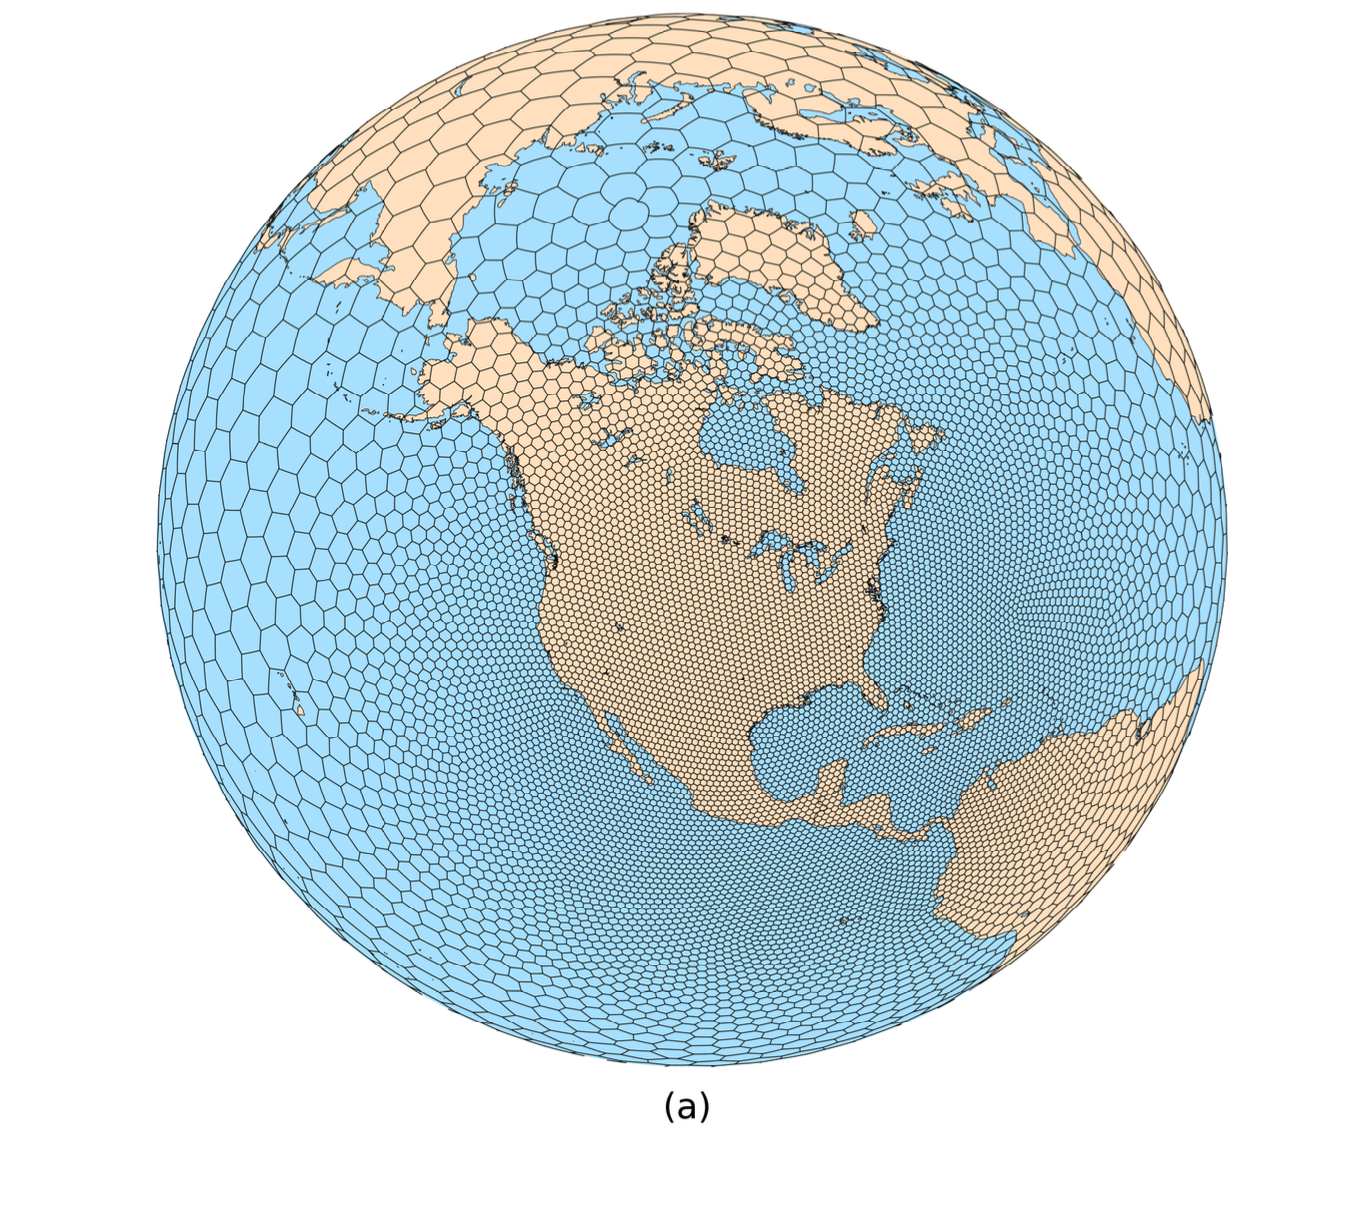
\includegraphics[width=0.7\textwidth, trim=10 70 10 0, clip]{docs/figuras/chapter3/ncl_plots_a.png} % Substitua pelo nome do seu arquivo
	\vspace{2mm}
	
	\centering 
	Source: \url{https://www2.mmm.ucar.edu/projects/mpas/site/visualization.html} (2025) .\par
	\label{fig:mpas-a} % Fonte centralizada
\end{figure}

As one can see, one of the big differences between MPAS and its predecessor, the WRF model, is that the model is discretized on centroidal Voronoi meshes using a C-grid staggering of the prognostic variables, allowing variable horizontal resolution, and also solving the equations of motion directly on these unstructured meshes (Skamarock, 2012). 

For our study, a set of variables was chosen to perform it. Table XXX indicates the variable name inside MONAN, alongside with the long name and the unit.


Total rainfall was computed by simply summing the variables rainnc and rainc for each lat/lon point. The wspd is the module of the squared sum of zonal and meridional winds at the first model level. From uzonal\_200hPa below, all variables are computed at the reference level pressure; for instance, uzona\_200hPa means the zonal wind at the pressure level of 200hPa.

\subsection{Initial condition generation}

To begin the integration process, Initial Conditions (IC) must be prepared by MPAS requirements (one could use the MPAS user guide for more details). We generated the initial conditions using the Weather Research \& Forecasting Model (WRF) Pre-Processing System (WPS), utilizing data obtained from ERA5, which we pre-processed with the WPS. These initial conditions were then uploaded into the MONAN IC folder and executed accordingly. For the IC sensitivity test, we also acquired a GRIB file from the Global Forecast System (GFS) model, a courtesy provided by Saulo R. Freitas, who already had the data available. The model will initially be set up with a global 30 km MPAS grid, with plans to modify this in future sections. It is important to note that a new IC will need to be created for each resolution.

\subsection{Post-processing}

Since the model output is generated on a non-structured grid, a post-processing step is necessary to map the native MPAS output to other meshes, enabling visualization on a standard lat/lon map. To achieve this, MONAN employs the convert-MPAS project. This approach utilizes a nearest-neighbor scheme to remap integer fields to the target grid, with additional information available at this link.

In this study, the Climate Data Operators (CDO) were also utilized to remap various datasets, including ERA5, GPM-IMERG, GPM-MERGIR, and GSMaP, as well as several forecasts (such as those simulated at 15km and 60km horizontal resolutions) to the MONAN forecasts.
